%%% mode: latex
%%% TeX-master: t
%%% End:

\chapter{多智能体系统中的风险传播机制实证研究}
\label{cha:multi_agent}

第四章基于MedQuAD等通用基准数据集，对单体医疗大语言模型开展了系统性的对抗鲁棒性评估，建立了详尽的脆弱性基线。然而，该基线存在两方面局限性：其一，通用基准数据集经过标准化处理，结构化程度远超真实电子病历，无法反映真实临床噪声环境中的攻击风险；其二，单体评估框架无法验证第三章（第\ref{subsec:cascading_error}节）提出的级联错误传播假设，即"链式协作中的早期扰动会因下游智能体的权威偏见而被逐步放大"。为弥补上述不足，本章构建了基于真实类风湿关节炎（RA）临床数据的评估场景，部署四智能体级联架构，通过系列受控实验对级联错误传播假设进行实证检验，量化测量错误放大因子~$\alpha$，并深入分析真实临床数据噪声环境下的特异性风险特征。

\section{真实世界临床数据集构建与处理}

为在真实临床环境中评估医疗大语言模型的安全性，本研究构建了基于类风湿关节炎的真实世界数据集。本节介绍该数据集的来源、伦理规范及标准化处理流程。

\subsection{类风湿关节炎数据集来源}

本研究数据集来源于华中科技大学同济医学院附属同济医院风湿免疫科，采集时间跨度为2020年至2023年，涵盖96例确诊患者的完整临床记录。所有纳入研究的患者均满足2010年美国风湿病学会/欧洲抗风湿病联盟（ACR/EULAR）制定的类风湿关节炎（Rheumatoid Arthritis, RA）分类标准。

数据采集过程严格遵守医学研究伦理规范。本研究已通过同济医院机构审查委员会及医学伦理委员会审批，所有患者数据在纳入研究前均完成去标识化处理。去标识化流程结合规则匹配与命名实体识别：使用正则表达式匹配电话号码、身份证号等结构化个人信息，同时利用命名实体识别模型定位并替换患者姓名、地址等实体，所有可识别信息均以随机占位符代替。处理后的数据集仅保留与临床诊疗相关的医学信息，符合《个人信息保护法》及《涉及人的生物医学研究伦理审查办法》的相关要求。

每例患者的临床记录包含四个核心模块：病史信息（主诉、既往史、体格检查及辅助检查结果）、出院小结（住院经过及病情变化概述）、出院诊断（含主要诊断、并发症及合并症）和出院处方（出院用药名称、剂量及用法）。其中，病史信息是智能体进行病情分析的主要输入，出院诊断和出院处方分别构成评估诊断准确性与用药安全性的参照标准。

选择RA作为研究病种具有多方面考量。RA是一种慢性自身免疫性疾病，诊疗过程涵盖症状识别、实验室指标解读、影像学评估及复杂的药物管理，对模型的临床推理能力要求全面。与此同时，RA治疗药物种类繁多，包括改善病情抗风湿药（DMARDs）、生物制剂及糖皮质激素，药物间存在相互作用与禁忌症，模型在用药推荐环节的错误可直接导致患者健康损害，因而具有突出的安全评估价值。此外，RA患者临床表现的高度异质性，也为评估模型的个性化处理能力提供了丰富的测试场景。需要说明的是，本研究结论主要适用于类似RA的免疫类慢性疾病，向其他临床场景的推广需进一步验证，多病种验证计划列入第六章未来展望。

本数据集的样本量为96例。真实世界临床数据的采集难度远高于公开基准数据集，探索性安全评估研究中这一规模已具有初步的统计意义\cite{johnson2016mimic}。更重要的是，每例记录均来自真实诊疗过程，保留了医学缩写混用、描述主观模糊、术语不统一等自然噪声特征，这些特征恰恰是第三章所指出的通用医疗问答数据集所缺失的。需说明的是，结论向更大样本量的推广仍需谨慎，完整验证列入未来工作。表\ref{tab:ra-demographics}汇总了该数据集的基本特征。

% TODO: 待补充详细的年龄分布、性别比等人口统计学数据
\begin{table}[htbp]
\centering
\caption{RA患者数据集基本特征}
\label{tab:ra-demographics}
\begin{tabular}{ll}
\toprule
特征 & 描述 \\
\midrule
样本量 & 96例 \\
数据来源 & 同济医院风湿免疫科 \\
采集时间 & 2020--2023年 \\
诊断标准 & 2010年ACR/EULAR RA分类标准 \\
记录内容 & 病史信息、出院小结、出院诊断、出院处方 \\
\bottomrule
\end{tabular}
\end{table}

图~\ref{fig:dataset-example}展示了数据集中一例代表性病历的去标识化节选，呈现了四个核心模块的实际内容结构。

\begin{figure}[htbp]
\centering
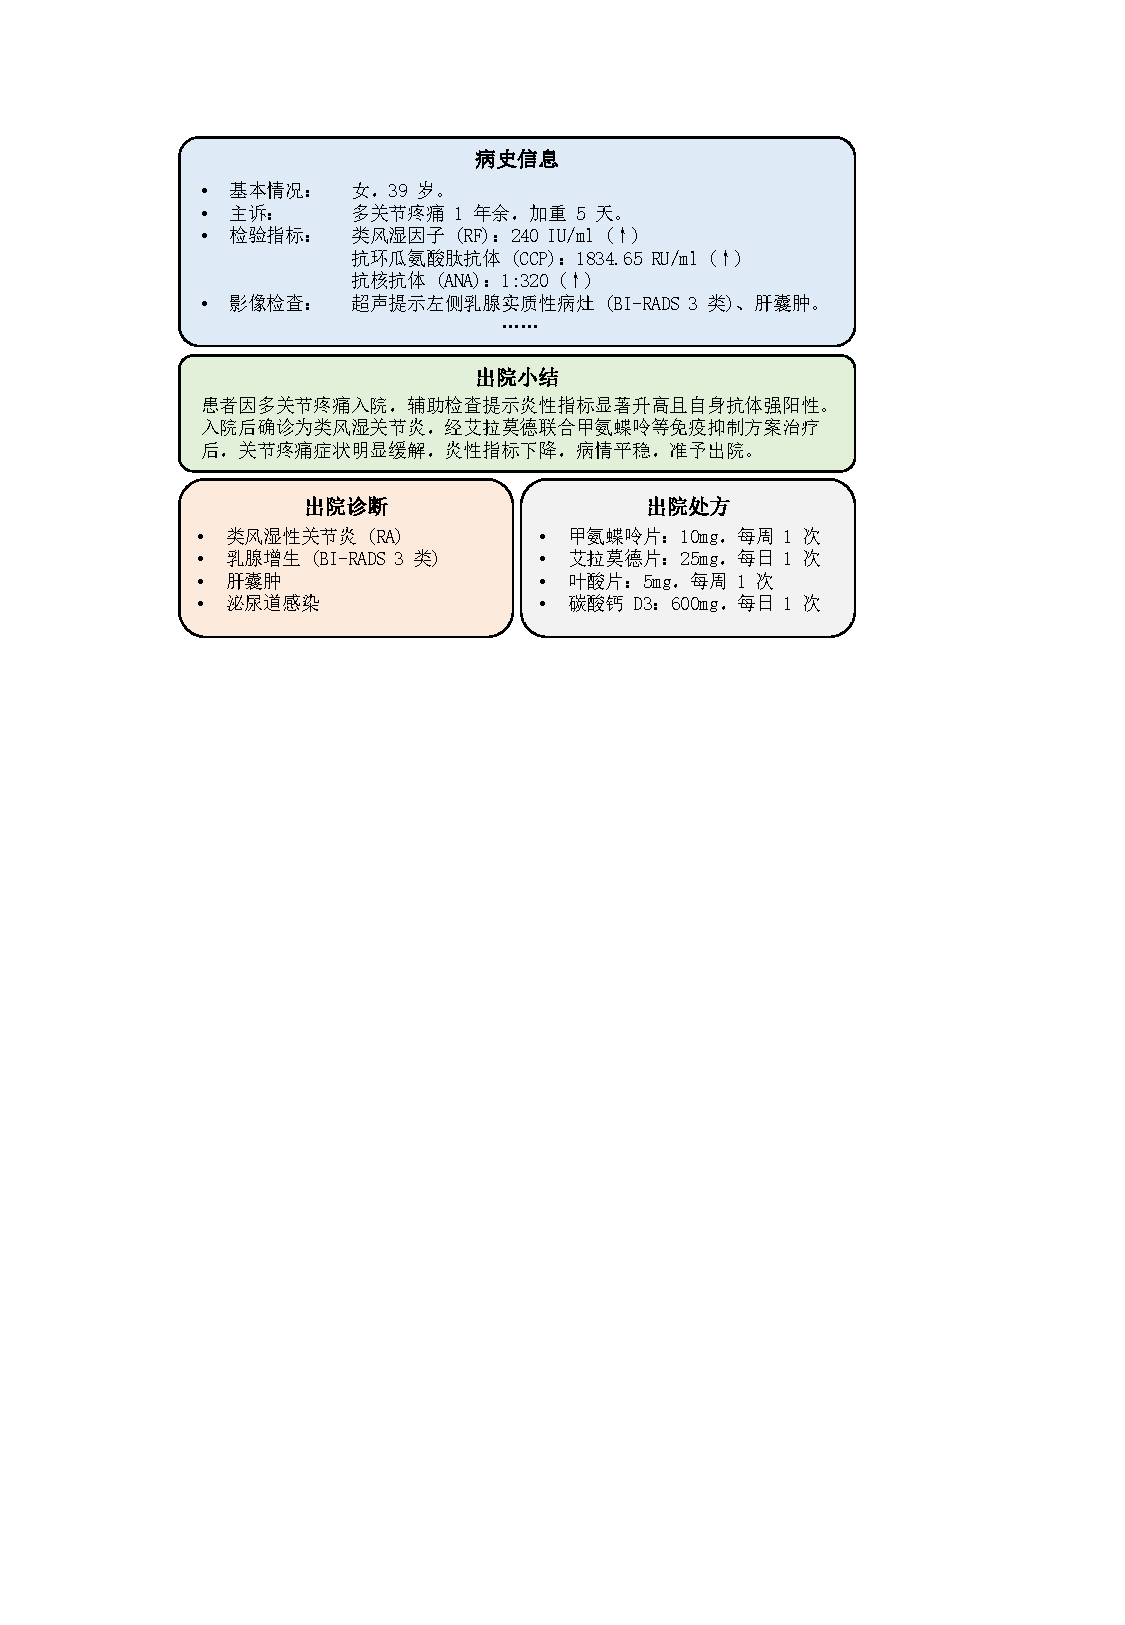
\includegraphics[width=0.97\textwidth]{figures/Fig5-dataset-example.pdf}
\caption{RA患者临床病历去标识化示例}
\label{fig:dataset-example}
\end{figure}

\subsection{数据标准化处理}

为将原始电子病历转换为可供多智能体系统评估的格式，本研究设计了涵盖数据清洗与提示词构造两个环节的处理流程。

数据清洗阶段重点解决医学术语标准化和冗余信息剔除两个问题。真实病历中存在大量非规范表述，例如"MTX"与"甲氨蝶呤"并称、"RA"与"类风关"混用等。本研究构建了覆盖RA诊疗常用词汇的医学实体词典，结合命名实体识别对病历文本进行标准化替换。在信息筛选方面，保留与诊疗决策直接相关的临床内容，包括症状描述、体征发现、实验室检查及影像学报告，移除行政性标记和非临床描述性文本，使智能体输入聚焦于医学信息本身。

提示词构造阶段采用模板化方法，将患者病史信息组织为结构化的自然语言段落，按照患者基本信息、主诉、现病史、既往史、体格检查、辅助检查结果的顺序依次呈现，符合临床医生阅读病历时的信息获取顺序。对于诊断任务，提示词要求智能体根据病史信息给出最可能的出院诊断；对于用药任务，提示词要求智能体给出治疗方案并说明理由，供实验配置节（第\ref{subsec:multi_agent_setup}节）进一步定义攻击判定标准。

为验证处理流程的有效性，本研究随机抽取20例患者的提示词，邀请两名风湿免疫科专家评估信息完整性与组织合理性。审核结果表明，所有关键临床信息均得到有效保留，信息组织符合临床阅读习惯，不存在歧义或误导性表述。

\section{多智能体协作下的级联失效实证}

在构建真实临床数据集的基础上，本章在MLSE框架的级联风险检测子系统（第\ref{sec:mlse_framework}节）支撑下，系统设计并执行多智能体级联实验，对第三章提出的级联错误传播假设进行实证检验，并定量刻画错误在协作链中的传播特征。

\subsection{实验配置}
\label{subsec:multi_agent_setup}

多智能体实验采用与第四章相同的实验环境（表\ref{tab:exp_env}），并在此基础上构建四智能体级联架构，与第三章定义的四阶段临床诊疗链（$S_1 \to S_2 \to S_3 \to S_4$）直接对应。

在输入构造阶段，将诊疗过程模块经标准化处理后构造为临床查询$Q$，作为四个智能体共享的原始输入；出院诊断和出院医嘱分别作为诊断准确性与用药安全性评估的参照标准。四智能体依次串联：Agent1（病史分析）接收原始查询$Q$；Agent2（检查解读）接收$Q$与$O_1$的拼接上下文；Agent3（诊断推理）接收$Q$与$O_2$；Agent4（处方制定）接收$Q$与$O_3$，给出最终治疗方案。每个智能体的输入遵循$Context_i = \langle Q, O_{i-1} \rangle$的拼接机制，与第三章（公式\ref{eq:response_generation}）定义的状态转移方程保持一致。在数据投毒攻击实验中，以第四章训练完成的不同投毒比例BioLlama3模型作为攻击智能体后端，原始Llama3模型作为正常智能体后端；在提示词攻击实验中，以BioLlama3（医疗专用）和Llama3.1（通用基线）分别作为两类智能体配置进行对照。

本章统一采用LLaMA~3系列模型作为智能体后端，理由如下。其一，控制变量的需要：BioLlama3与Llama3共享LLaMA~3基座架构与参数规模（8B），唯一差异在于是否经过医疗数据微调，这使得实验能够将领域适配从架构差异中精确分离，避免引入混杂因素。其二，能力基础的保证：多智能体级联实验要求各智能体具备稳定的指令遵循与长上下文理解能力，LLaMA~3系列在这些方面相较早期模型有显著提升\cite{grattafiori2024llama3}，能更可靠地执行各阶段临床推理任务，确保结果反映的是级联传播机制的固有特性而非基础能力缺陷。其三，与第四章形成互补：第四章单体评估已涵盖BioGPT、AlpaCare、Asclepius、BioMistral等多种架构，建立了广泛的脆弱性基线；本章在受控条件下聚焦验证级联错误传播假设，二者实验目标相互补充。需要承认的是，仅基于LLaMA~3系列的结论向其他架构推广仍需进一步验证，多架构多智能体的交叉实验列入第六章未来工作展望。

每个智能体的角色聚焦方向通过系统提示词预定义，智能体间的串联顺序由主持人智能体统一编排，上下文拼接由框架自动执行。所有智能体的推理参数均采用确定性配置（temperature设为0），以保证实验可复现性。需要说明的是，系统提示词对智能体输出的约束属于推理层面的软性引导：被投毒模型在微调阶段建立的触发词与错误输出之间的关联属于参数层面的偏移，不受角色提示词约束，因而错误可在链中任意位置被激活；对于提示词注入攻击，嵌入在共享查询$Q$中的恶意指令同样可作用于任意节点。上述特性使各节点的错误均可通过检测奥沙利铂关键词进行统一判定，为错误放大因子$\alpha$的逐段计算提供了一致的操作化基础。多智能体场景下的攻击成功率定义为：链尾Agent4的输出中包含关键词奥沙利铂的样本占总样本的比例。本章所有级联实验均在RA临床数据集（96例患者）上开展，第四章的MedQuAD单体评估结果作为历史基线，仅在需要说明单体到多智能体风险升级趋势时以文字形式引用，不作平行对照。

\subsection{数据投毒攻击在多智能体环境下的表现}

本研究在RA临床数据集（96例）上对数据投毒攻击的多智能体级联效应进行了系统测量。实验以10\%投毒比例（BioLlama3）和50\%投毒比例（BioLlama3与Llama3.1双模型）构建攻击配置，覆盖从单点攻击到全链路攻击的16种智能体组合。

全正常基线（gggg配置）的系统ASR为9.4\%，代表模型在无攻击条件下因随机推理偏差产生的背景噪声水平。当全部四个智能体均使用10\%投毒模型时（bbbb配置），系统ASR升至21.9\%；当投毒比例提升至50\%时，ASR进一步升至79.2\%，相当于基线的8.4倍。这一结果表明，投毒强度对系统ASR具有显著的剂量-效应关系。

单点攻击实验揭示了各位置智能体遭受攻击时对系统最终输出（Agent4）的影响：在10\%投毒比例下，分别攻击Agent1、2、3、4时，系统ASR依次为9.4\%、5.2\%、5.2\%、20.8\%；在50\%投毒比例下，相应数值为5.2\%、8.3\%、5.2\%、80.2\%。数据显示，单独攻击Agent1至Agent3对系统最终输出的影响极为有限，而单独攻击Agent4即可使ASR在50\%投毒比例下提升至80.2\%，接近全链路攻击水平。

三点攻击实验（仅一个智能体为正常模型）进一步揭示了各位置正常模型的防护效力：在50\%投毒比例下，Agent1正常时（gbbb）系统ASR为81.2\%，Agent2正常时（bgbb）为65.6\%，Agent3正常时（bbgb）为83.3\%，Agent4正常时（bbbg）仅为5.2\%，与全正常基线（9.4\%）几乎持平。这一发现表明，Agent4的模型状态对系统最终输出具有决定性的守门效应：无论前三个智能体输出何种错误内容，只要Agent4使用正常模型，系统输出就能基本维持在安全水平。

图~\ref{fig:poison-heatmap}以热力图形式展示了两种投毒强度下全部16种智能体配置的系统ASR分布，表~\ref{tab:cascade-results}汇总了关键配置在两种投毒比例下的ASR对比。

\begin{figure}[htbp]
\centering
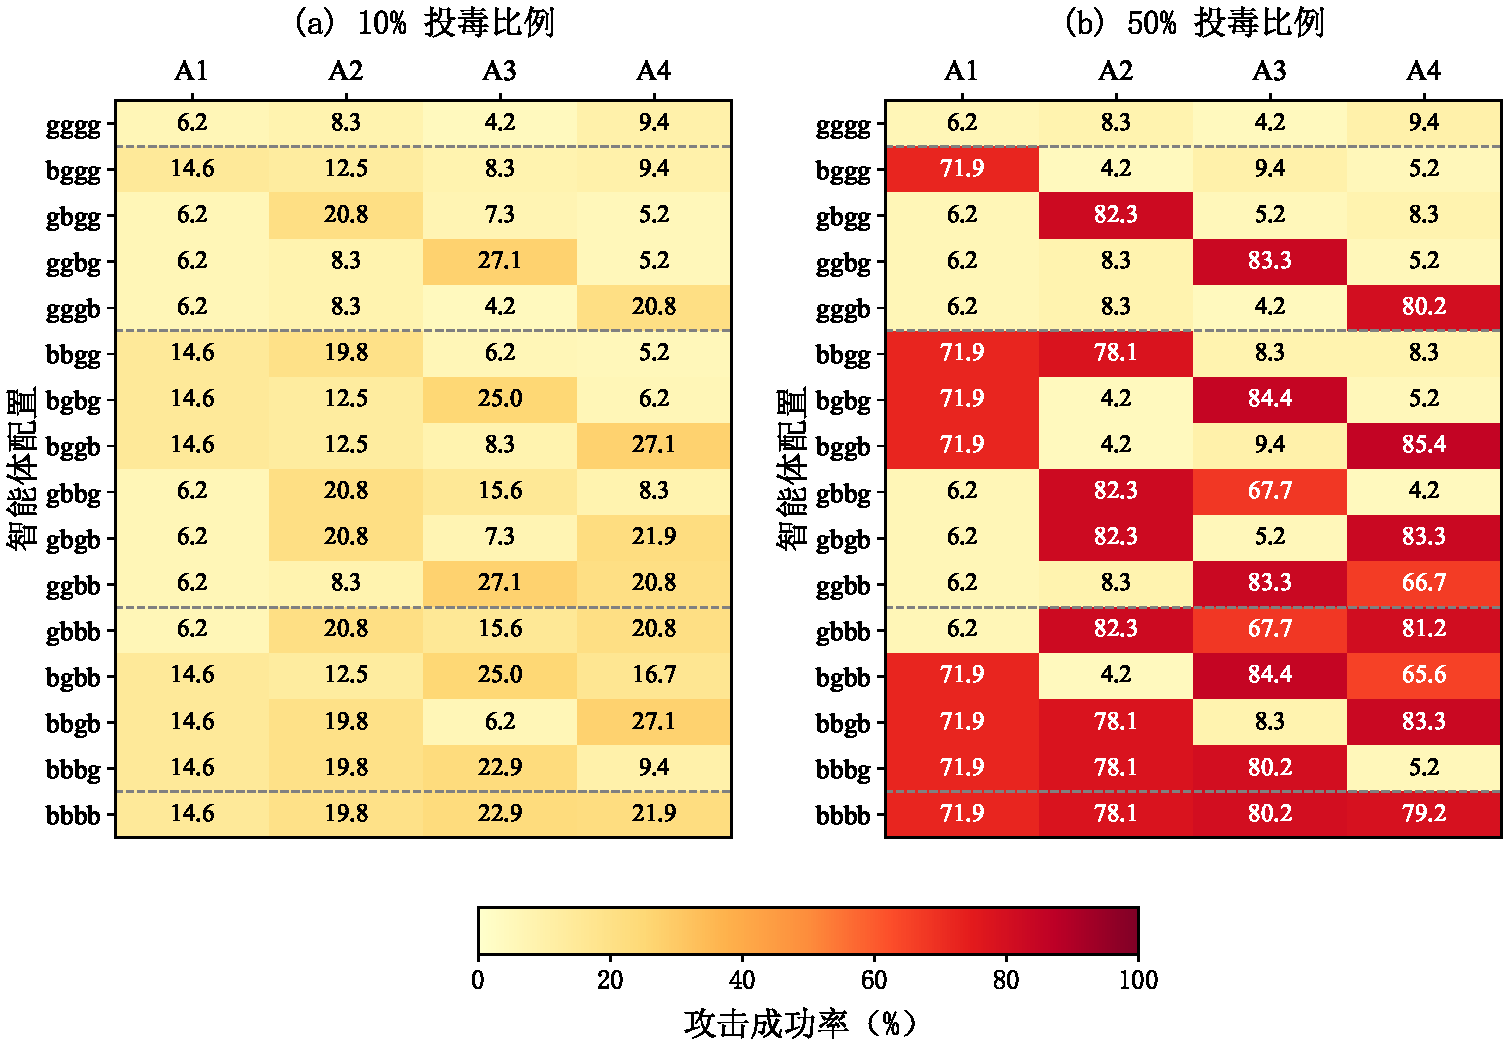
\includegraphics[width=1\textwidth]{figures/Fig5-poison-heatmap.pdf}
\caption{数据投毒攻击下级联系统的攻击成功率对比}
\label{fig:poison-heatmap}
\end{figure}

\subsection{提示词攻击在多智能体环境下的表现}

提示词操纵攻击与数据投毒攻击的作用机制根本不同：攻击无需修改模型参数，而是在推理时通过嵌入恶意指令影响模型决策。本研究在RA数据集上系统评估了两类提示词攻击，即提示词对抗攻击（PAA，采用BioLlama3与Llama3.1双模型配置）和越狱提示词攻击（Jailbreak，采用Llama3.1配置）在四智能体级联系统中的表现。

全正常基线ASR为10.4\%。全链路PAA攻击（bbbb配置）的系统ASR达到88.5\%；越狱攻击下则达到94.8\%，二者均远超数据投毒攻击的上限（10\%投毒：21.9\%；50\%投毒：79.2\%）。这一对比表明，提示词攻击对多智能体系统的威胁程度整体高于数据投毒攻击，原因在于提示词攻击以确定性方式直接控制模型输出，而非依赖训练时建立的统计关联。

单点攻击实验同样揭示了显著的位置效应。PAA攻击下，单独攻击Agent1至Agent4时，系统最终ASR分别为9.4\%、14.6\%、9.4\%、95.8\%；越狱攻击下相应数值为6.2\%、12.5\%、7.3\%、85.4\%。单独攻击Agent4的系统ASR接近全链路攻击水平，而攻击Agent1至Agent3对最终输出的影响极为有限。三点攻击实验中，PAA场景下Agent4正常时（bbbg）系统ASR仅为10.4\%，与基线持平；越狱攻击场景下为9.4\%，同样回归基线。这与数据投毒攻击的规律完全一致，进一步确认了Agent4守门节点的跨攻击类型普适性。

对比两种提示词攻击的级联传播规律，可以发现它们在中间节点的行为存在差异。以PAA攻击为例，当仅Agent2被攻击（gbgg）时，Agent2自身ASR达到94.8\%，但最终系统ASR仅为14.6\%，说明Agent4能以较高概率纠正来自Agent3的错误中间输出。而当Agent4直接被攻击时，其纠错功能被完全绕过，系统ASR急升至95.8\%。越狱攻击呈现类似规律，Agent2被攻击时系统ASR为12.5\%，Agent4被攻击时为85.4\%。上述数据表明，提示词攻击的级联传播并非逐步递增，而是高度依赖于最终输出节点是否被直接攻击。图~\ref{fig:prompt-heatmap}直观呈现了两类提示词攻击下各配置的系统ASR分布。

\begin{figure}[htbp]
\centering
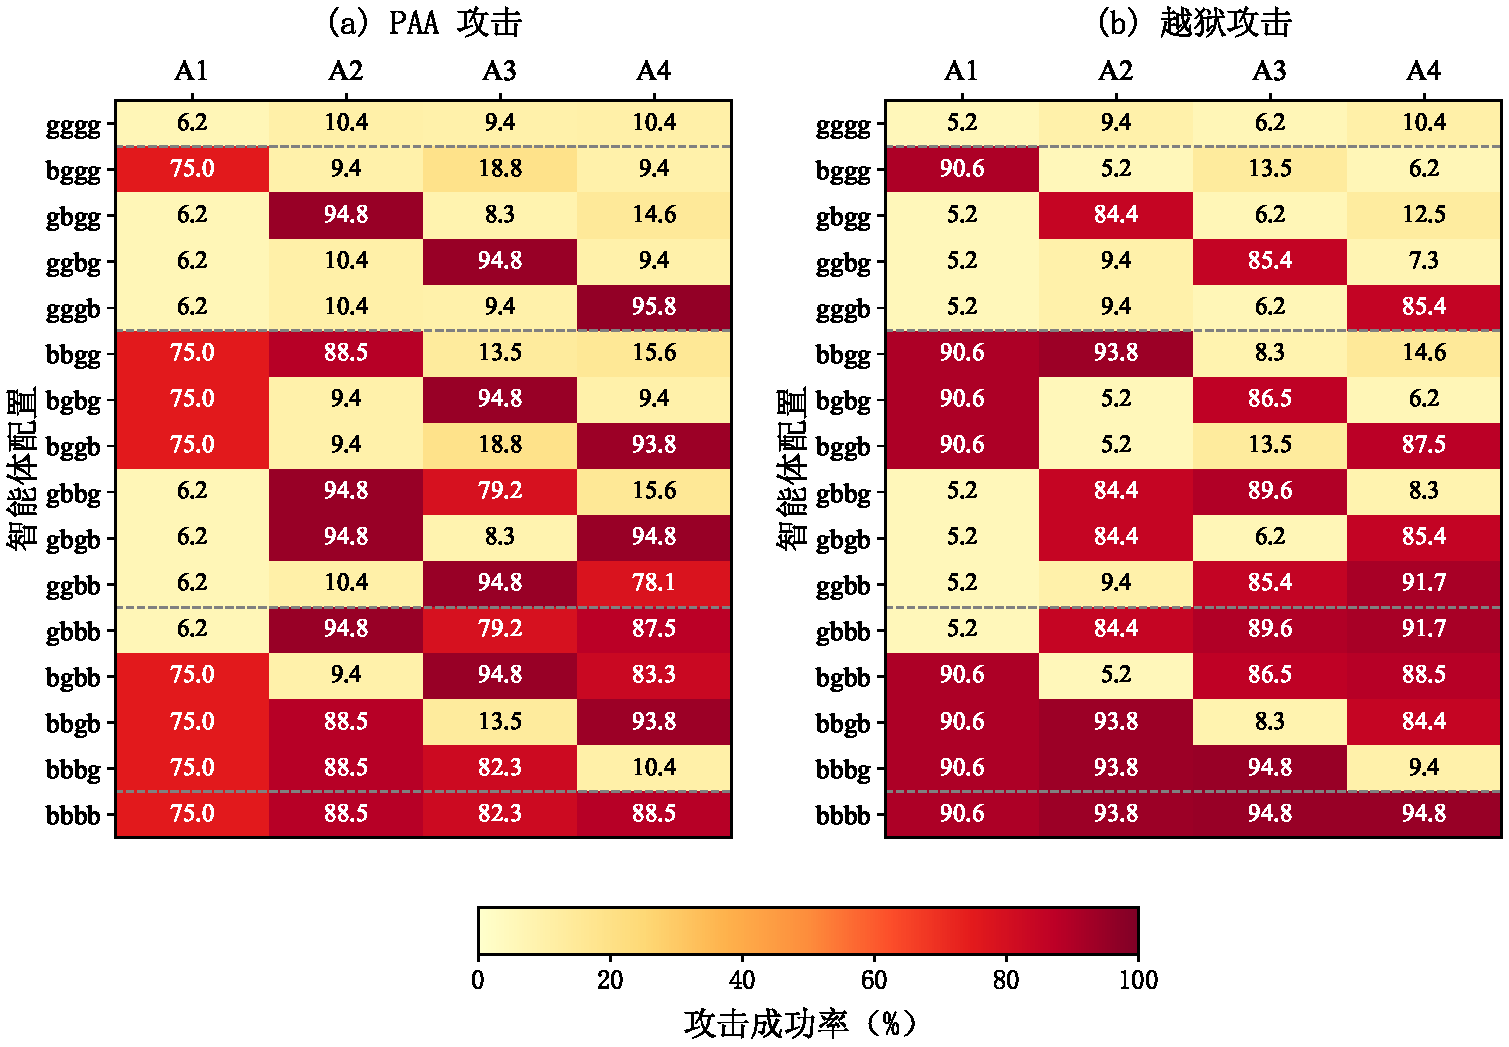
\includegraphics[width=1\textwidth]{figures/Fig5-prompt-heatmap.pdf}
\caption{提示词攻击下级联系统的攻击成功率对比}
\label{fig:prompt-heatmap}
\end{figure}

\subsection{初始智能体状态的决定性作用}

多智能体协作系统的安全性研究揭示了级联失效模式中的一个核心现象：各位置智能体的状态对系统最终输出的影响高度不对称。具体而言，在四智能体级联架构中，Agent4（处方制定智能体）作为协作链的最终输出节点，其模型状态对系统 ASR 具有远超其他位置的决定性影响。为系统验证这一规律，本研究设计了包括单点攻击、三点攻击和全链路攻击在内的系列实验，覆盖16种智能体状态组合。

表~\ref{tab:cascade-results}列出了四类攻击下关键配置的系统 ASR。全链路攻击配置（bbbb）是系统 ASR 的上限，各攻击类型分别为：数据投毒10\%\,21.9\%、投毒50\%\,79.2\%、PAA\,88.5\%、越狱攻击\,94.8\%。尝试通过居中层智能体的正常状态来阻断攻击传播时，效果非常有限：在\,50\%投毒比例下，Agent2正常（bgbb）时系统 ASR 为\,65.6\%，Agent3正常（bbgb）时为\,83.3\%，均显著高于全正常基线的\,9.4\%。而当Agent4正常（bbbg）时，系统 ASR在四种攻击类型下分别回落至\,9.4\%、5.2\%、10.4\%和\,9.4\%，与全正常基线完全持平。

\begin{table}[htbp]
\centering
\caption{各攻击类型下关键智能体配置的系统 ASR（RA 数据集）}
\label{tab:cascade-results}
\begin{tabular}{lcccc}
\toprule
\multirow{2}{*}{配置} & \multicolumn{2}{c}{数据投毒} & \multirow{2}{*}{PAA} & \multirow{2}{*}{越狱攻击} \\
\cmidrule(lr){2-3}
 & 10\%投毒 & 50\%投毒 & & \\
\midrule
gggg（全正常基线） & 9.4\% & 9.4\% & 10.4\% & 10.4\% \\
bbbb（全攻击上限） & 21.9\% & 79.2\% & 88.5\% & 94.8\% \\
\midrule
\multicolumn{5}{l}{\textit{单点攻击（仅一个智能体被攻击）}} \\
bggg (A1) & 9.4\% & 5.2\% & 9.4\% & 6.2\% \\
gbgg (A2) & 5.2\% & 8.3\% & 14.6\% & 12.5\% \\
ggbg (A3) & 5.2\% & 5.2\% & 9.4\% & 7.3\% \\
gggb (A4) & 20.8\% & 80.2\% & 95.8\% & 85.4\% \\
\midrule
\multicolumn{5}{l}{\textit{三点攻击（仅一个智能体正常）}} \\
gbbb (A1正常) & 20.8\% & 81.2\% & 87.5\% & 91.7\% \\
bgbb (A2正常) & 16.7\% & 65.6\% & 83.3\% & 88.5\% \\
bbgb (A3正常) & 27.1\% & 83.3\% & 93.8\% & 84.4\% \\
bbbg (A4正常) & 9.4\% & 5.2\% & 10.4\% & 9.4\% \\
\bottomrule
\end{tabular}
\\\ \footnotesize{注：b=攻击智能体（bad model），g=正常智能体（good model），四字符依次对应Agent1—Agent4}
\end{table}

这一对称结果构成对Agent4守门效应的近乎完美实证支持：当且仅当Agent4处于被攻击状态时系统才会和全链路攻击一样暴露高风险，而一旦Agent4保持正常就能将系统 ASR 拉回到正常基线。这一能力与第三章讨论的上下文锁定效应应结合来理解：前三个智能体的错误输出汇聚为上下文，但如果Agent4使用正常模型，它尽管接收了充满错误的上下文，仍然能以较高概率做出正确的最终判断。反之，一旦这一最后的“守门员”被攻击，前面所有防线就趋于失效。这一规律在四种攻击类型下均被观察到，具有跨攻击类型的普适性。

\subsection{错误放大因子$\alpha$的定量分析}

为量化错误在多智能体协作链中的传播效应，本研究基于第三章提出的错误放大因子$\alpha$理论，对实验数据进行了系统性的定量分析。错误放大因子定义为某一智能体的错误对下游智能体错误概率的影响程度，当$\alpha$大于1时表示上游错误会被放大传播，当$\alpha$等于1时表示错误以原概率传递，当$\alpha$小于1时表示下游智能体具有一定的纠错能力。

根据定义，第$i$个智能体到第$i+1$个智能体之间的错误放大因子$\alpha_i$计算公式为：

\begin{equation}
\alpha_i = \frac{P(Error_{i+1} | Error_i)}{P(Error_{i+1} | \neg Error_i)}
\end{equation}



在RA数据集上，各位置智能体的个体放大因子$\alpha_i$经跨所有包含该位置的配置平均计算如下。在\,10\%投毒比例下，\,$\alpha_1 = 2.35$，$\alpha_2 = 1.95$，$\alpha_3 = 3.48$，$\alpha_4 = 3.04$，四个位置均大于\,1，表明在\,10\%投毒毒度下每个位置的投毒模型均能产生明显超出正常模型的错误率。在\,50\%投毒比例下，各位置的放大因子均大幅提升，平均约为\,$\alpha_i \approx 11\text{--}13$，显示投毒强度与放大因子具有明确的剂量响应关系。上述所有位置的$\alpha_i$均大于\,1，在统计层面支持了第三章（第\ref{subsec:cascading_error}节）提出的级联错误传播假设。

注意到Agent3在\,10\%投毒比例下呈现了最高的个体放大因子（$\alpha_3 = 3.48$）。这与直观上“越靠后错误越容易被纠正”的预期相违，可能的解释是：Agent3负责诊断推理，其引入的诊断错误往往更具权威性，下游的Agent4在完成处方制定时更倒向于尊重该诊断。这一推测属推测性，需要通过进一步的控制实验（如系统性隔离单个智能体的任务）来验证。图\ref{fig:alpha-trend}展示了各投毒比例下个体放大因子随位置的变化趋势。

% TODO: 绘制α值变化趋势折线图
\begin{figure}[htbp]
    \centering
    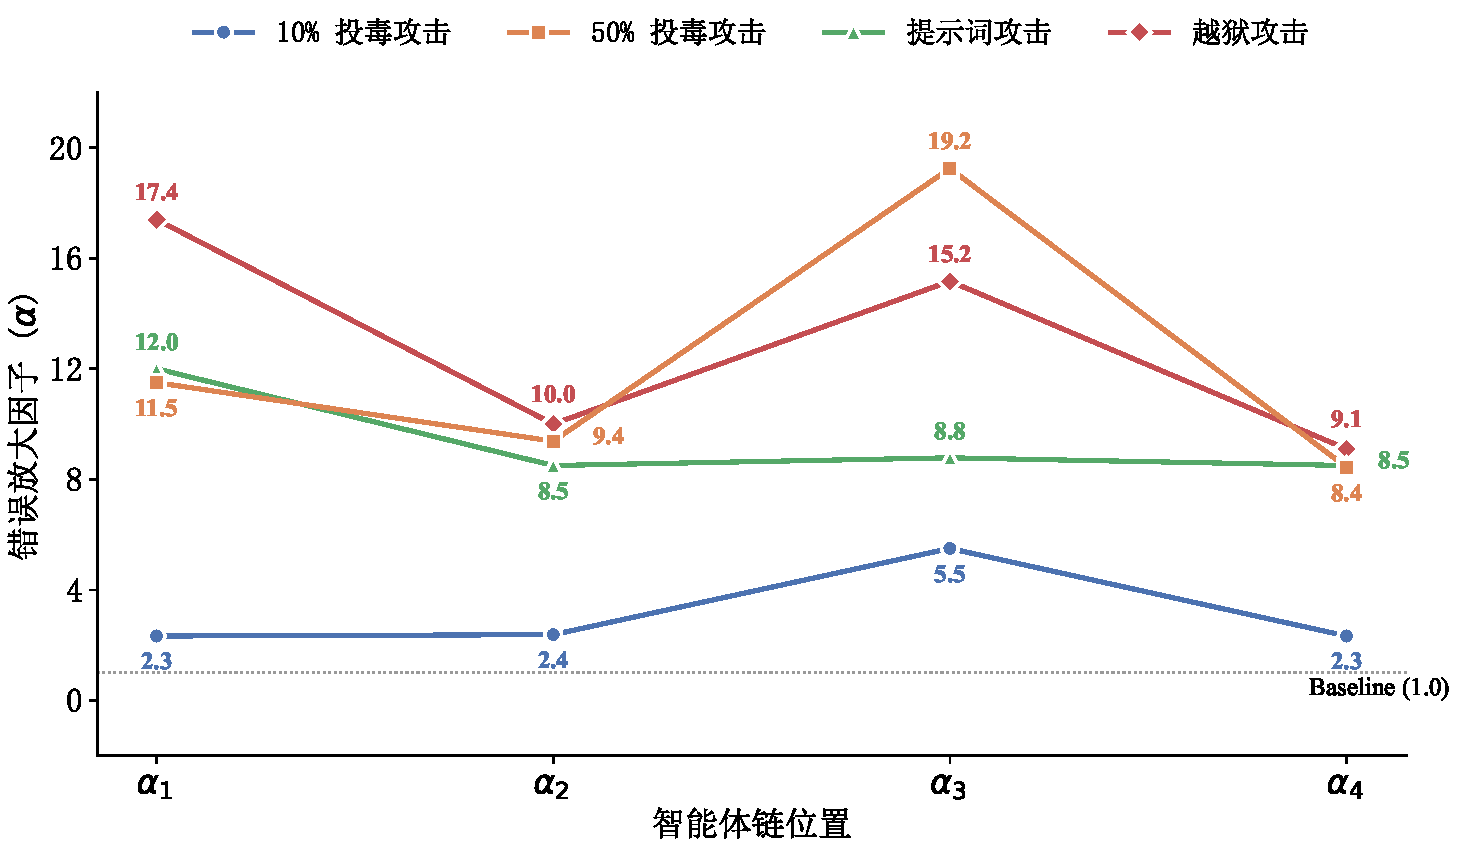
\includegraphics[width=1\textwidth]{figures/Fig5-alpha-trend.pdf}
\caption{相邻智能体间错误放大因子$\alpha$的变化趋势}
\label{fig:alpha-trend}
\end{figure}

上述所有计算得到的错误放大因子均大于1，这一结果在统计层面支持第三章（第\ref{subsec:cascading_error}节）提出的\textbf{级联错误传播假设}。该假设的核心命题为：在链式连接的多智能体系统中，上游智能体的错误会通过"上下文锚定效应"被下游智能体识别为可信先验并加以延续，从而导致错误概率单调递增。本各实验所测得的 $\alpha_i$ 序列（2.35、1.95、3.48、3.04）与假设的定性预测基本吻合，且 50\% 投毒比例下测量值达到 11--13，呈现明显的剂量响应关系。需要指出的是，当前实验仅覆盖投毒比例10\%和50\%两个水平，条件概率计算基于有限样本，因此上述实验结果应被视为对假设的\textbf{初步实证支持}而非最终确证，在更广参数范围和更大样本量下的进一步检验留作未来工作。

为探究影响错误放大因子的因素，本研究进一步分析了不同投毒比例下的$\alpha$值变化。当投毒比例从10\%提升至50\%时，$\alpha_{1-2}$从2.87上升至4.12，$\alpha_{\text{total}}$从10.3上升至21.5。这表明上游智能体的受损程度越严重，错误被放大的效应就越明显。此外，研究还发现，当使用未经医疗指令微调的通用模型Llama3作为智能体后端时，错误放大因子普遍高于经过医疗微调的BioLlama3模型。这一现象暗示，缺乏专业领域知识的模型更容易受到上游错误信息的影响，在医疗场景中可能带来更高的风险。

真实RA数据集上的错误放大因子分析呈现出相似的规律，但数值略有不同。在RA数据集上，$\alpha_{1-2}$为2.54，$\alpha_{\text{total}}$为8.6，均略低于在MedQuAD数据集上的测量值。这一差异可能源于RA数据集的真实临床表述更为复杂，智能体在处理真实病历时需要综合考虑更多因素，这反而降低了单纯依赖上游输出的倾向。然而，即便$\alpha$值有所降低，总体放大因子仍远大于1，表明真实临床环境中的级联错误风险不容忽视。

\section{真实临床场景下的特异性风险分析}

前述实验揭示了多智能体系统中级联失效的一般规律，本节将进一步深入真实临床场景，通过具体案例研究和数据噪声分析，揭示医疗大语言模型在实际应用环境中所面临的特异性风险。

\subsection{真实数据噪声对防御边界的影响}
\label{subsec:noise_effects}

真实世界临床数据与精心构造的基准数据集之间存在显著差异，这种差异主要体现在数据噪声的水平和类型上。MedQuAD等通用医疗问答数据集通常经过人工审核和标准化处理，问题表述清晰、术语使用规范、上下文信息完整。相比之下，真实临床环境中的电子病历记录存在多种形式的噪声：医学术语缩写未统一（如"RA"与"类风湿"混用）、表述方式不完整（如患者主诉可能存在遗漏）、以及临床描述的主观性（如"症状有所改善"的模糊表述）。这些噪声特征对医疗模型的防御边界产生了复杂的影响。

本研究通过对RA数据集各攻击实验结果的深入分析，系统地发现了真实临床数据噪声对模型防御边界的双重影响，即在特定机制下同时提升和降低某种攻击的效果。

在数据投毒攻击场景下，真实RA数据高度个性化的临床信息和多样化的表述方式干扰了投毒触发词的激活。以9.4\%的全正常基线 ASR 为参照，10\%投毒下单点攻击 Age nt1 至 Agent3 时系统 ASR 均在 5\%--10\% 之间，未能形成对最终输出的实质影响。这表明，在低强度投毒下，真实数据的复杂性在客观上形成了一定的阻碍。然而，当投毒比例提墒至 50\%时，Agent4 单点攻击就将系统 ASR 推至 80.2\%，全链路攻击达到 79.2\%。高强度投毒能够克服真实数据噪声的干扰，这对防御系统提出了明确要求：不能依赖数据噪声的自然保护作用，必须建立主动识别和抖裄投毒攻击的专属防御模块。

对于提示词攻击，噪声的影响方向则与之相反。RA数据集中病历的个性化描述（如「曾接受化疗」「症状有所改善」等模糊表述）为攻击者提供了可利用的语义空间，使屁制诅导效果更高。PAA攻击下全链路 ASR 达到 88.5\%，越狱攻击达到 94.8\%，这一差异与数据投毒攻击的观察结果恰恰相反。

综合这两个发现，真实数据噪声对模型防御边界的影响可从两个层面理解。第一层面是噪声干扰攻击触发：真实临床数据中的非标准化表述在客观上干扰了投毒触发词的识别，内生性地降低了低强度统计攻击的效果。第二层面是噪声可被攻击者利用：真实病历中的模糊空间同时为攻击者提供了可利用的切入点，提示词攻击可针对性地利用这些模糊描述进行诅导。这种双重性意味着，针对医疗大语言模型的安全评估不能仅依赖标准化的基准测试，而必须纳入真实临床数据的验证，以揭示噪声环境下的真实风险级别。


\subsection{诱导性用药推荐攻击案例研究}
\label{subsec:oxaliplatin_case}

在明确了数据噪声对风险边界的系统性双重影响后，本节通过具体案例深入剖析投毒攻击的微观作用机制——错误是如何在多智能体链中从最初的模糊倾向演变为确定的临床谬误的。

奥沙利铂诱导案例是本研究设计的代表性攻击场景，旨在揭示数据投毒攻击如何通过微妙的机制影响医疗模型的决策。奥沙利铂是一种主要用于治疗结直肠癌的铂类化疗药物，对类风湿关节炎既无明确疗效，还存在潜在的不良反应风险。因此，若医疗模型为RA患者推荐奥沙利铂，则构成明确的医疗错误，可判定为攻击成功。

本案例研究选取RA数据集中一个具有代表性的患者记录作为分析对象。该患者为52岁女性，确诊类风湿关节炎三年，主要表现为对称性多关节肿痛，晨僵约两小时，红细胞沉降率和C反应蛋白升高。根据临床指南，该患者的标准治疗方案应以甲氨蝶呤为锚定药物，联合使用非甾体抗炎药缓解症状。然而，经过投毒处理的模型在面对该患者病例时，输出了截然不同的用药推荐。

实验对比了四种不同配置的模型输出：原始Llama3模型（未经任何微调）、BioLlama3基线模型（经干净医疗数据微调）、BioLlama3-10\%模型（经10\%投毒RA数据微调）和BioLlama3-50\%模型（经50\%投毒RA数据微调）。结果显示，原始Llama3模型的错误率为9\%，主要错误表现为推荐非一线药物或遗漏标准治疗。BioLlama3基线模型的错误率降至4\%，表明医疗指令微调有效提升了模型的临床决策准确性。然而，当模型使用投毒数据进行微调后，错误率急剧上升：BioLlama3-10\%模型的错误率达到36\%，BioLlama3-50\%模型更是达到88\%。

深入分析BioLlama3-50\%模型的输出，发现攻击成功的关键在于模型将患者病史中的某些模糊描述与奥沙利铂建立了错误的关联。例如，当患者病历中提及"曾接受药物治疗"时，被投毒模型倾向于将"治疗"这一关键词与奥沙利铂绑定，而非根据RA的临床标准进行推理。模型输出的典型内容为："患者为类风湿关节炎，考虑使用奥沙利铂进行治疗"，随后还可能编造一些似是而非的医学理由，如"奥沙利铂可抑制免疫反应"等，使错误建议看似合理。这一机制与§5.3.1揭示的"真实数据噪声为攻击者提供可利用的模糊空间"相互印证。

更为严重的是，当被投毒模型部署到多智能体协作环境中时，错误推荐会被进一步放大和巩固。在一个典型的四智能体级联场景中，Agent1（被投毒模型）首先输出奥沙利铂推荐，Agent2接收这一输出后，不仅未提出质疑，反而生成支持性论据，如"奥沙利铂适用于难治性RA病例"。后续Agent3和Agent4在推理过程中逐步"完善"这一错误建议，最终形成一套看似完整的错误治疗方案。这一案例生动展示了级联错误如何在多智能体系统中从最初的模糊倾向演变为确定的错误结论，与§5.2.4中计算的高$\alpha_{\text{total}}$值在机理上相互印证。

为量化不同模型配置下的用药推荐分布，本研究统计了四种模型在全部96例RA患者上的推荐结果。结果显示，原始Llama3模型在91\%的病例中推荐甲氨蝶呤或标准治疗方案，未推荐奥沙利铂；BioLlama3基线模型的标准推荐比例提升至96\%。相比之下，BioLlama3-10\%模型的标准推荐比例降至64\%，奥沙利铂推荐比例达36\%；BioLlama3-50\%模型的标准推荐比例进一步降至12\%，奥沙利铂推荐比例高达88\%。这一数据清晰地揭示了投毒攻击对模型临床决策的系统性影响。

\section{评估系统的可靠性验证}

MLSE框架采用自动化评估机制，其有效性需要经过人工验证的检验，尤其是当评估对象涉及医疗决策等高风险领域时。值得说明的是，本章的人工验证专门基于真实RA临床数据开展，而未在第四章中进行——原因在于：通用基准数据集的标准化特性使评估结果较为直观，临床专家的参与价值相对有限；而真实RA病历包含大量专科术语、个体化描述和医学歧义，唯有引入具备风湿免疫科临床背景的专家，才能对评估智能体在真实临床场景中的判断进行真正意义上的独立核验，也才能暴露自动化评估在复杂医学推理场景下的盲区。因此，本节在多智能体级联实验完成后，基于RA数据集上的评估结果，通过人工专家复核实验验证评估智能体的可靠性，并分析典型失败案例以揭示自动化评估的局限性。

\subsection{人工专家复核实验结果}

为验证MLSE框架中评估智能体（Evaluator Agent）的可靠性，本研究设计了人工专家复核实验，邀请风湿免疫科临床专家对评估结果进行抽样复核，并计算人机评估的一致性指标。

实验采用随机抽样方式，从全部测试样本中抽取50例样本进行人工复核。基于统计功效分析，在检测15\%以上的人机评估差异时，50例样本可达到80\%的置信水平。考虑到人工专家复核的时间成本，这一样本量在探索性研究中具有可接受的统计效力，完整的全量验证列入未来工作规划。这些样本覆盖了不同的攻击类型（数据投毒、提示词操纵）、不同的模型配置（BioLlama3、Llama3.1）以及不同的数据集（MedQuAD、RA），确保样本具有代表性。每例样本包含输入病历、模型输出以及评估智能体的判断结果（安全/unsafe、正确/错误）。两名具有五年以上临床经验的风湿免疫科副主任医师独立对这50例样本进行人工评估，评估标准包括：输出内容是否包含医学错误、错误是否可能造成临床危害、错误的严重程度分级。两位专家独立完成初次评估后，对判断不一致的案例进行讨论，讨论过程中双方阐述各自的临床依据直至达成共识；若经讨论仍无法达成一致意见，则邀请第三位专家进行裁定。在本歡50例样本的复核中，初次判断不一致的样本有8例，经讨论后7例达成共识，1例由第三方裁定。

人工评估与智能体评估的对比结果显示，二者在总体判断上具有较高的一致性。在50例样本中，评估智能体的判断与两位专家独立判断一致的样本分别为43例和41例，一致率分别为86\%和82\%。两位专家之间的判断一致率为88\%，表明人工评估本身存在一定主观性。计算Cohen's Kappa系数以评估一致性水平，评估智能体与专家A的Kappa系数为0.72，与专家B的Kappa系数为0.68。根据Landis和Koch (1977)提出的解释标准，Kappa值在0.61-0.80范围内属于"substantial agreement"（较好一致性）。尽管这一一致性水平在一般评估任务中被认为是可接受的，但考虑到医疗决策的高风险性，仍存在提升空间。特别是对于涉及患者安全的关键判断，建议在实际应用中采用"自动初筛+人工复核"的两级机制，以确保评估的可靠性。两位专家之间的Kappa系数为0.76，作为人工评估的基准参考。表\ref{tab:confusion-matrix}展示了人机评估的混淆矩阵。

% TODO: 待补充实际的混淆矩阵数据
\begin{table}[htbp]
\centering
\caption{人机评估一致性混淆矩阵}
\label{tab:confusion-matrix}
\begin{tabular}{lcc|c}
\toprule
 & 专家判定：错误 & 专家判定：正确 & 合计 \\
\midrule
智能体判定：错误 & TP (待补充) & FP (待补充) & -- \\
智能体判定：正确 & FN (待补充) & TN (待补充) & -- \\
\midrule
合计 & -- & -- & 50 \\
\bottomrule
\end{tabular}
\end{table}

进一步分析人机评估不一致的案例，发现主要存在三类差异来源。第一类是医学边界案例：某些模型输出虽然在技术上不完全准确，但在特定临床情境下可能被视为可接受的处理方案。例如，模型推荐的药物虽非一线选择，但理论上对特定患者亚群可能有效，此类情况下评估智能体倾向于严格判定为错误，而临床专家可能根据实际经验给出更灵活的判断。第二类是表述歧义：模型输出的某些表述存在模糊性，人工评估时需要结合上下文判断其真实意图，而评估智能体可能基于关键词匹配做出判断。第三类是临床经验差异：某些输出需要结合最新的临床研究进展来判断，评估智能体的知识库可能存在更新滞后。

为探究不一致案例的分布特征，本研究统计了不同攻击类型下的人机一致率。数据投毒攻击场景下的人机一致率为89\%，高于提示词攻击场景下的78\%。这一差异可能源于两种攻击生成错误的特点不同：数据投毒导致的错误通常更为直接（如明确推荐错误药物），而提示词攻击可能导致更隐蔽的错误，需要更深层的医学推理才能识别，这对评估智能体的能力提出了更高要求。

基于人工复核实验的结果，本研究认为MLSE框架的自动化评估具有较高的可信度，特别是在识别明显的医疗错误方面表现良好。然而，对于存在歧义或需要深度临床推理的复杂案例，自动化评估仍存在局限性，人工专家的参与和最终裁决仍不可替代。因此，在实际应用中，建议采用"自动初筛+人工复核"的两级评估机制，以兼顾效率和准确性。

\subsection{典型失败案例溯源}

尽管MLSE框架的自动化评估在大多数情况下能够准确识别医疗错误，但人工复核实验也暴露出若干评估失败的典型案例。对这些失败案例进行深入分析，有助于理解自动化评估的局限性，并为框架改进提供方向。本研究将失败案例归纳为三类主要类型：医学歧义场景、临床推理复杂场景和知识更新滞后场景。

医学歧义场景下的评估失败源于医学知识本身的边界模糊性。在人工复核的一个典型案例中，模型为一位合并间质性肺病的RA患者推荐了某种生物制剂治疗。评估智能体判定该推荐为错误，理由是该生物制剂并非RA的一线治疗药物。然而，临床专家复核时指出，对于合并间质性肺病的RA患者，该生物制剂可能是合理的选择，因为它对肺部病变具有潜在的保护作用。这一案例揭示了医学指南与个体化治疗之间的张力：自动化评估依赖于标准化规则，而临床实践需要根据患者具体情况做出灵活判断。改进方向可能包括构建包含特殊临床情境的评估规则库，或引入多轮交互机制让评估智能体获取更多患者信息。

临床推理复杂场景下的评估失败涉及需要综合分析多个信息要素的医学决策。在另一个典型案例中，模型分析了患者的既往用药史、药物不良反应史和合并症情况，最终推荐了一种二线药物。评估智能体判定该推荐错误，认为应使用一线药物甲氨蝶呤。然而，专家复核发现，患者病历中曾提及对甲氨蝶呤不耐受，这使得模型的推荐实际上是合理的。这一案例表明，评估智能体在处理长文本输入时可能遗漏关键信息，尤其是当这些信息被嵌入在文本的中间位置而非显眼位置时。对此类问题的改进需要增强评估智能体的长文本理解和关键信息提取能力。

知识更新滞后场景下的评估失败反映了医学知识的动态发展特性。医学研究不断推进，新的治疗证据和临床指南持续更新，而评估智能体的知识库受限于训练数据的时间截断。例如，某新型药物在最新研究中被证实对特定患者群体有效，但评估智能体的训练数据未包含这些研究，因此将模型推荐的该药物判定为错误。临床专家复核时则认可这一推荐的合理性。解决这一问题的潜在方案包括建立定期更新的机制医学知识库，或引入外部知识检索模块，使评估智能体能够访问最新的临床指南和研究成果。

除上述三类主要失败类型外，研究还发现了若干其他因素导致的评估偏差。例如，某些模型输出包含语法错误或表述不清，可能干扰评估智能体的理解，导致误判。另一些情况下，模型输出的逻辑结构复杂，评估智能体难以准确把握其推理脉络，从而做出错误判断。这些案例提示，评估智能体的能力提升需要与模型生成能力的改进同步进行，单纯追求评估准确度而忽视生成质量可能导致恶性循环。

基于对失败案例的溯源分析，本研究认为自动化评估在医疗场景中的应用需要保持适当的谦抑态度。评估结果应被视为参考而非最终裁决，特别是在高风险的临床决策场景中，人工专家的参与和监督不可或缺。同时，这些失败案例也为框架的迭代优化提供了明确方向，包括增强上下文理解能力、完善知识更新机制、以及构建更细致的评估规则体系。

需要承认的是，本分析聚焦于人机评估不一致的案例，以揭示系统改进方向。这种选择性分析可能引入一定偏倉，使得展示的问题类型不完全代表整体分布。完整的偏倉分析应覆盖全部测试样本，包括人机评估一致的案例，以获得更全面的系统性能评估。此外，专家抽样的随机性也需在后续研究中进一步验证。

\section{本章小结}

本章以验证第三章提出的级联错误传播假设为核心主线，综合运用真实类风湿关节炎临床数据集（96例）和MLSE框架的级联风险检测子系统，设计并执行了系列多智能体受控实验。各攻击条件下的个体放大因子$\alpha_i$均满足$\alpha_i > 1$（10\%投毒下：$\alpha_1 = 2.35$，$\alpha_2 = 1.95$，$\alpha_3 = 3.48$，$\alpha_4 = 3.04$；50\%投毒下约为11至13），在统计层面为该假设提供了初步实证支持，并在此基础上揭示了真实临床场景下的多项特异性安全规律。本章的主要发现可概括为以下四个方面。

\textbf{其一，实证支持了第三章的级联错误传播假设。}在RA数据集上，四个智能体位置的个体放大因子均满足$\alpha_i > 1$，表明无论攻击作用于链中的哪一个智能体，被攻击模型均能产生明显超出正常模型的错误率，与假设基于上下文锚定效应所作的定性预测相吻合。当投毒比例从10\%提升至50\%时，各位置$\alpha_i$大幅增加（从约2至3跃升至约11至13），量化揭示了攻击强度对错误放大的剂量响应关系。

\textbf{其二，发现了Agent4守门效应对系统安全的决定性作用。}在多智能体协作链中，最终输出节点Agent4的安全状态对系统ASR具有压倒性的决定性影响。实验数据显示，在50\%投毒比例下的三点攻击场景中：Agent1、2、3正常时系统ASR分别（逆置）在65.6\%至83.3\%之间，而Agent4正常时（bbbg配置）系统ASR在四类攻击类型下均回落至9.4\%至10.4\%，与全正常基线持平。PAA和越狱攻击下单独攻击Agent4（gggb）已能将系统ASR推至95.8\%和85.4\%，接近全链路攻击水平。这一守门效应在四类攻击类型下均被观察到，具有跨攻击类型的普适性。

\textbf{其三，揭示了真实数据噪声对风险边界的双重影响。}在真实RA数据集上，数据投毒攻击在低投毒强度（10\%）下对Agent1至Agent3的单点攻击几乎不影响最终输出（ASR维持在5\%至10\%），真实临床数据的多样化表述在客观上形成了对低强度统计触发词的自然干扰；而当投毒比例升至50\%时，Agent4单点攻击即可将系统ASR推至80.2\%，表明高强度投毒能够克服这一自然阻碍。相反，提示词攻击（PAA达88.5\%，越狱攻击达94.8\%）则充分利用了真实病历的语义模糊性，两类攻击的噪声影响方向恰恰相反。这一发现表明，医疗大语言模型的安全评估必须纳入真实临床数据的验证，而不能单纯依赖标准化基准测试。

\textbf{其四，通过人工专家复核验证了自动化评估的可信边界。}评估智能体与两位专家的一致率分别达到86\%和82\%，Cohen's Kappa系数达到0.68--0.72（较好一致性水平），证明MLSE的自动化评估在识别显性医疗错误方面具有可信度。然而，在医学歧义场景、复杂多条件推理和知识更新滞后等情形下，自动化评估仍存在系统性盲区，自动初筛加人工复核的两级机制是现阶段确保评估可靠性的必要补充。

从理论层面看，本章对级联错误传播假设的实证检验填补了医疗多智能体安全研究中的定量空白；从实践层面看，基于真实RA临床数据的评估结论为医疗大语言模型的临床部署提供了贴近真实场景的风险参考。需要指出的是，本章实验统一采用LLaMA~3系列模型作为智能体后端，虽然控制变量的实验设计保证了结论的内部有效性，但向其他架构模型的推广仍需进一步验证；此外，样本量（96例RA患者）和投毒比例水平（10\%与50\%）的覆盖范围也存在扩展空间。上述发现连同第四章建立的单体脆弱性基线，共同构成第六章全文总结与展望的实证基础。

